\subsection{To-do list} \label{To-do list}
%\begin{figure}[H]
%	\centering
%	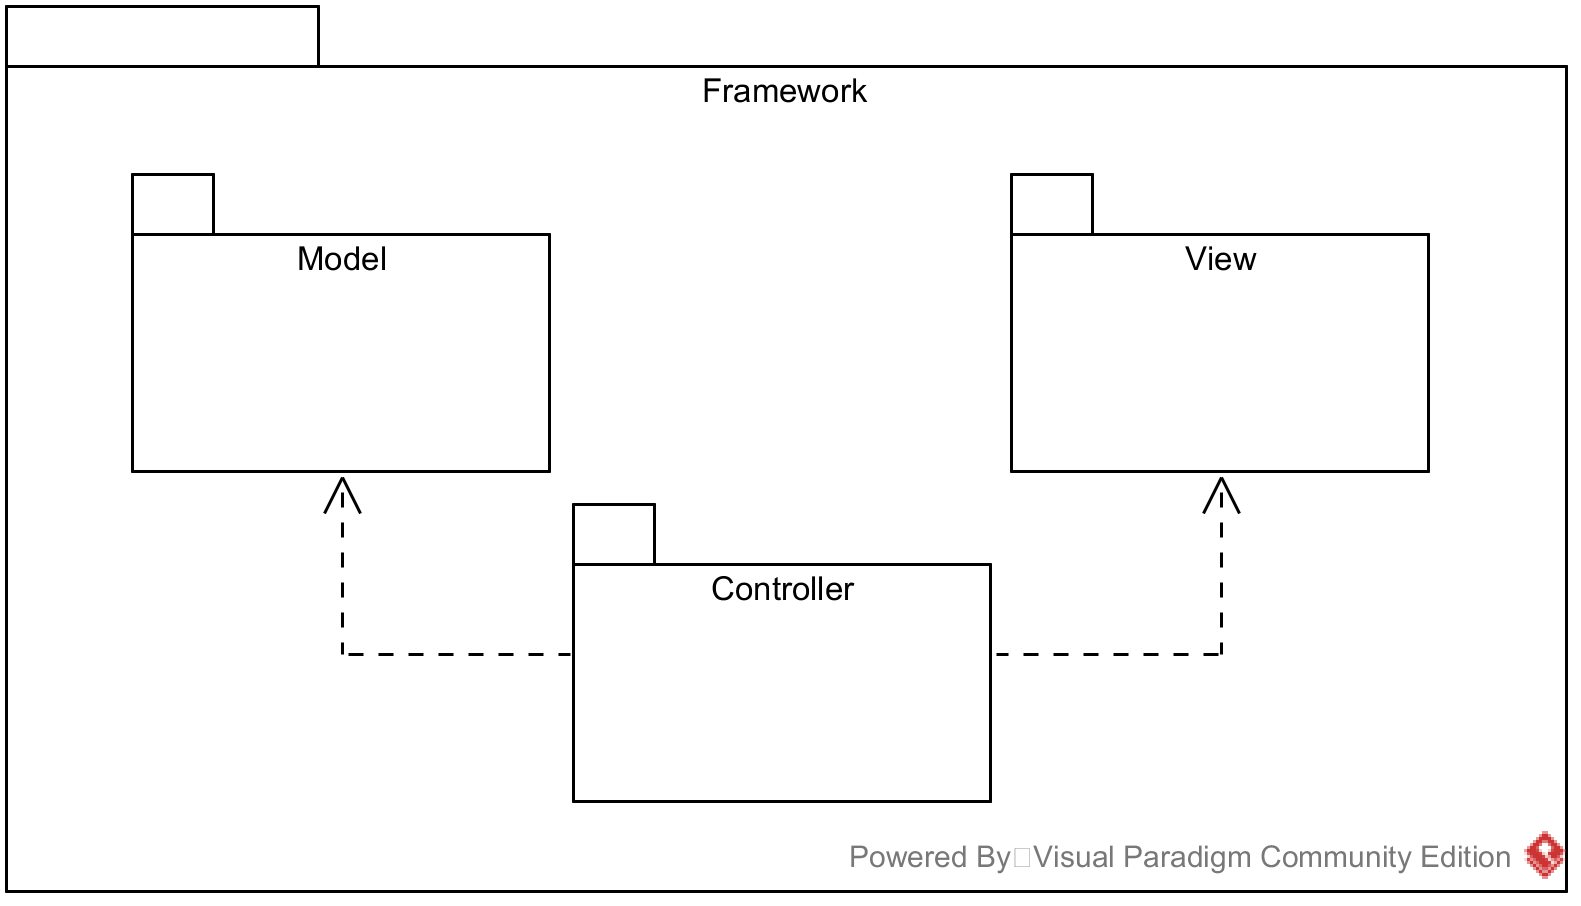
\includegraphics[width=15cm]{./diagrammi/framework.png}
%	\caption{Componente Framework}
%\end{figure}
\glossario{TodoList} è il package base per la prima delle due demo. Come il framework segui il design pattern MVC ed è quindi composto dai package Model, View e Controller.

\setclass{TodoList::Model}
\subsubsection[::Model]{\class} \label{\class}
%\begin{figure}[H]
%	\centering
%	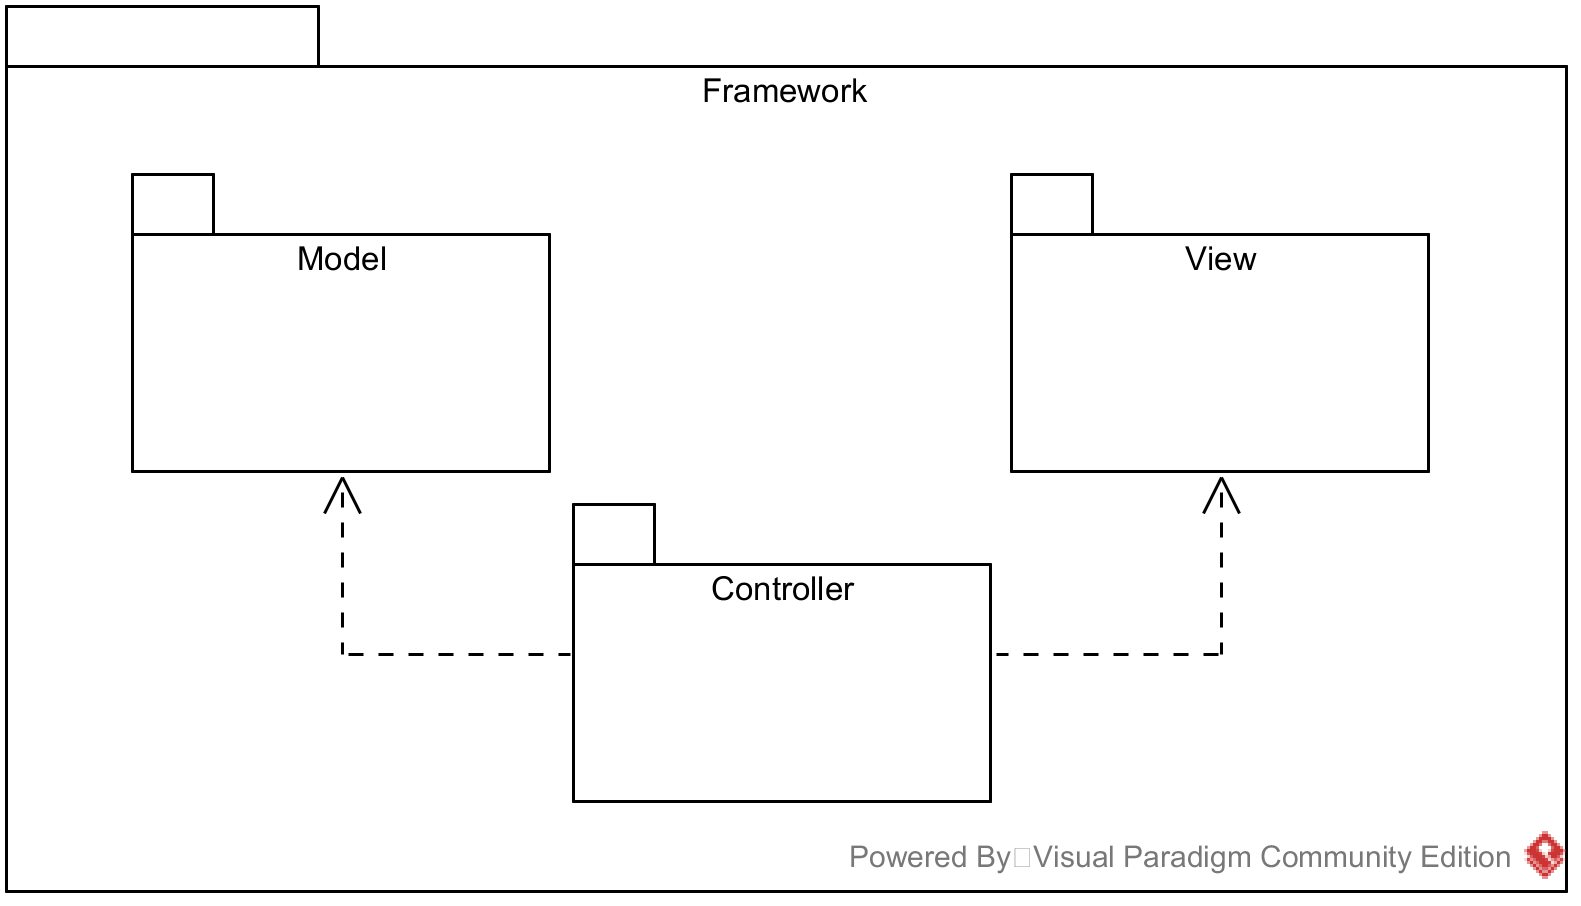
\includegraphics[width=15cm]{./diagrammi/framework.png}
%	\caption{Componente Framework}
%\end{figure}
Il package Model contiene i dati della To-do list ed è composto a sua volta dalle classi ListItem e ItemsStore.


\setclass{TodoList::Model::ListItem}
\subparagraph[::ListItem]{\class}\mbox{}\\ \label{\class}
%\begin{figure}[H]
%	\centering
%	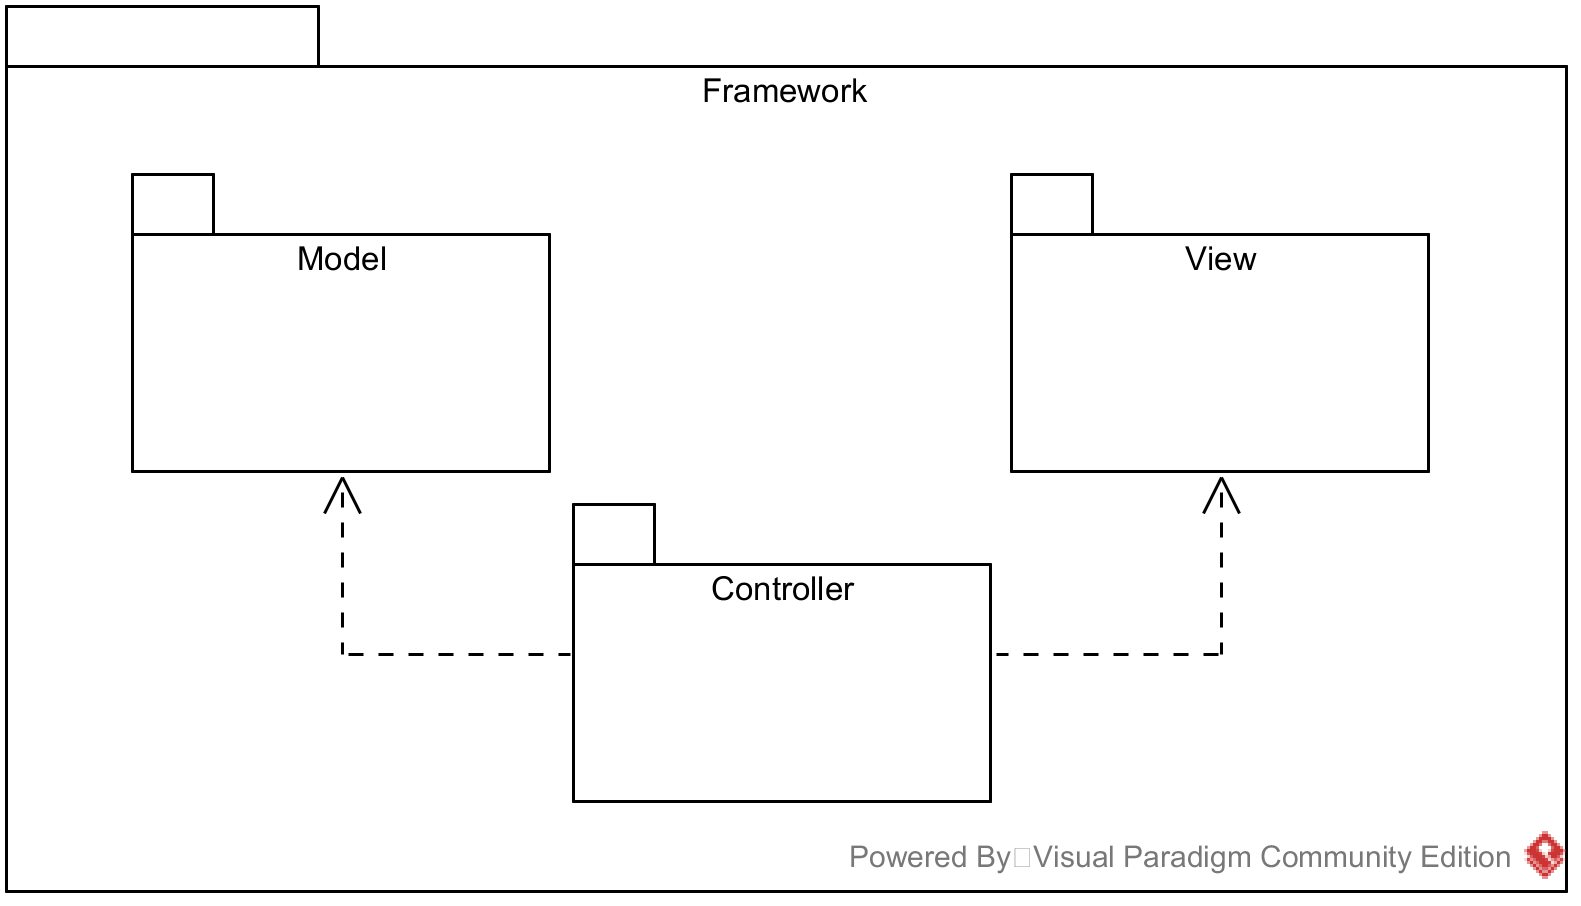
\includegraphics[width=15cm]{./diagrammi/framework.png}
%	\caption{Componente Framework}
%\end{figure}
\textbf{Descrizione:}
ListItem rappresenta un singolo elemento della lista To-do list.

\textbf{Utilizzo:}
Viene utilizzata per rappresentare gli elementi della To-do list.

\textbf{Attributi:}
\begin{itemize}
	\item \field{-id: string}: id unico identificativo dell'elemento;
	\item \field{-text: string}: testo dell'elemento;
	\item \field{-checked: bool}: stato dell'elemento: 
	\begin{itemize}
		\item true: completato;
		\item false: non completato.
	\end{itemize}
\end{itemize}

\textbf{Metodi:}
\begin{itemize}
	\item \method{+listItem(id:string, text:string)}: costruttore della classe;
	\begin{itemize}
		\item \param{id:string}: input dell'identificativo unico dell'elemento;
		\item \param{text:string}: testo dell'elemento;
	\end{itemize}
	\item \method{-setChecked()}: modifica lo stato dell'elemento per indicarlo come completato.
\end{itemize}

\setclass{TodoList::Model::ItemsStore}
\subparagraph[::ItemsStore]{\class}\mbox{}\\ \label{\class}
%\begin{figure}[H]
%	\centering
%	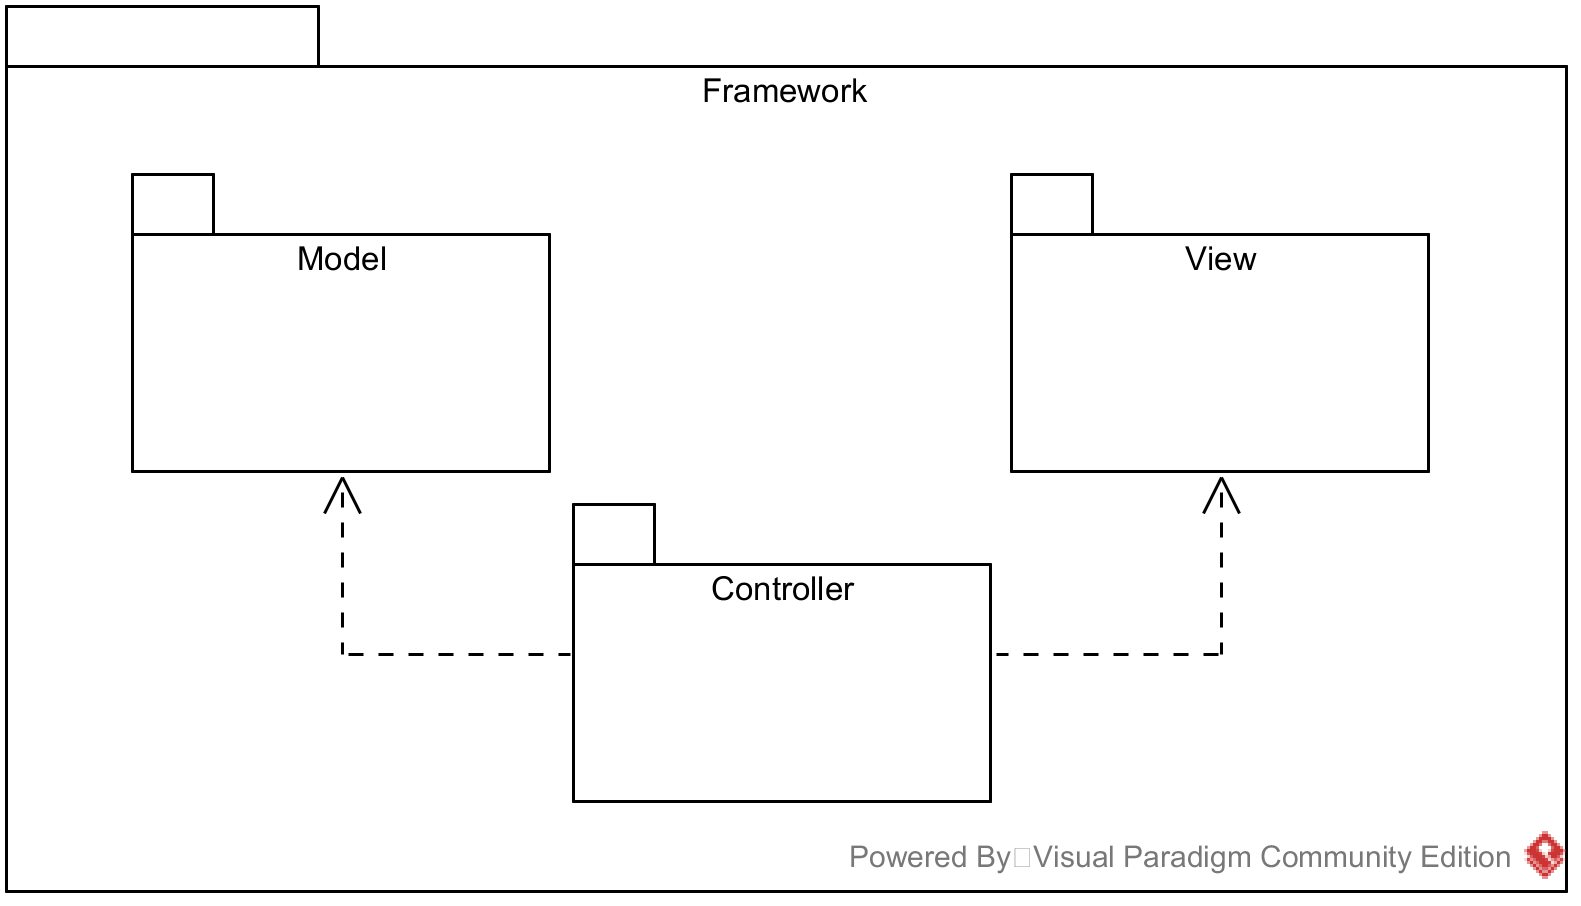
\includegraphics[width=15cm]{./diagrammi/framework.png}
%	\caption{Componente Framework}
%\end{figure}
\textbf{Descrizione:}
ItemsStore implementa la classe BubbleMemory e gestisce i dati della To-do list.

\textbf{Utilizzo:}
Viene utilizzata per gestire gli elementi della To-do list.

\textbf{Classi ereditate:}
\begin{itemize}
	\item \code{BubbleMemory}.
\end{itemize}

\textbf{Attributi:}
\begin{itemize}
	\item \field{-items: listItem[]}: array contenente gli elementi della lista;
\end{itemize}

\textbf{Metodi:}
\begin{itemize}
	\item \method{+ItemsStore():void}: costruttore della classe, crea l'array degli elementi della lista;
	\item \method{-addItems(item:listItem):void}: aggiunge un elemento alla lista;
		\begin{itemize}
			\item \param{item:listItem}: nome dell'elemento da aggiungere alla lista.
		\end{itemize}
	\item \method{-removeItems(id:string):void}: rimuove l'elemento identificato da id dalla lista;
		\begin{itemize}
			\item \param{id:string}: id dell'oggetto da rimuovere.
		\end{itemize}
	\item \method{-completeItems(id:string):void}: indica come completato l'elemento id;
		\begin{itemize}
			\item \param{id:string}: id dell'oggetto da indicare come completato.
		\end{itemize}
	\item \method{+getItems():listItem[]}: restituisce tutti gli elementi della lista;
	\item \method{+GetCompleted():object[]}: restituiscce tutti gli elementi completati della lista;
	\item \method{+handleActions(action:object):void}: effettua l'azione richiesta.
		\begin{itemize}
			\item \param{action:object}: azione che si vuole venga effettuata, può essere di tre tipi:
			\begin{itemize}
				\item ADD\_ITEM: indica la richiesta di aggiunta di un oggetto;
				\item REMOVE\_ITEM: indica la richiesta di rimozione di un oggetto;
				\item COMPLETE\_ITEM: indica la richiesta di indicare come completato un oggetto.
			\end{itemize}
		\end{itemize}
\end{itemize}

\setclass{TodoList::View}
\subsubsection[::View]{\class} \label{\class}
%\begin{figure}[H]
%	\centering
%	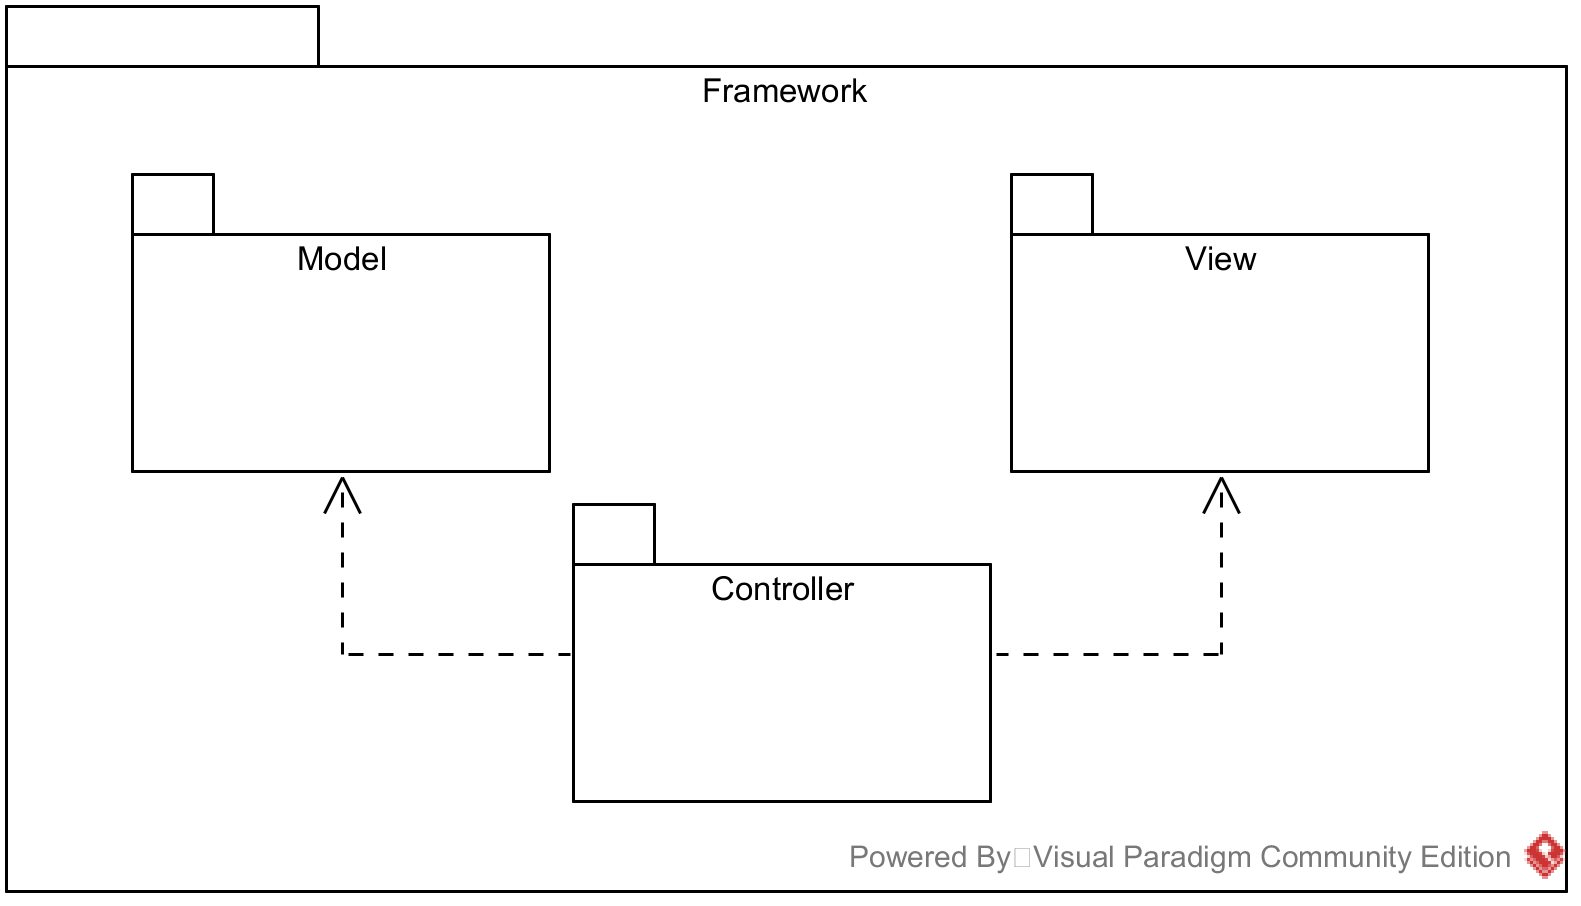
\includegraphics[width=15cm]{./diagrammi/framework.png}
%	\caption{Componente Framework}
%\end{figure}
Il package View si occupa di gestire la parte grafica della To-do list, ed è composto dalla classe listItemView.

\setclass{TodoList::View::listItemView}
\subparagraph[::listItem]{\class}\mbox{}\\ \label{\class}
%\begin{figure}[H]
%	\centering
%	\includegraphics[width=15cm]{./diagrammi/demo/todo-list/listitem.png}
%	\caption{Componente Framework}
%\end{figure}
\textbf{Descrizione:}
Questa classe gestisce la visualizzazione degli elementi della To-do list.

\textbf{Utilizzo:}
Viene utilizzata per gestire la view della To-do list.

\textbf{Classi ereditate:}
\begin{itemize}
	\item \code{React.Component}.
\end{itemize}

\textbf{Attributi:}
\begin{itemize}
	\item \field{-props: Object[]}: array contenente le proprietà degli elementi della lista.
\end{itemize}

\textbf{Metodi:}
\begin{itemize}
	\item \method{+ListItem(props: Object[])}: costruttore della classe, assegna le proprietà:
	\begin{itemize}
		\item \param{props: Object[]}: array contenente le proprietà degli elementi.
	\end{itemize}
	\item \method{+render(): React.Component}: renderizza il componente.
\end{itemize}

\setclass{TodoList::Controller}
\subsubsection[::Controller]{\class} \label{\class}
%\begin{figure}[H]
%	\centering
%	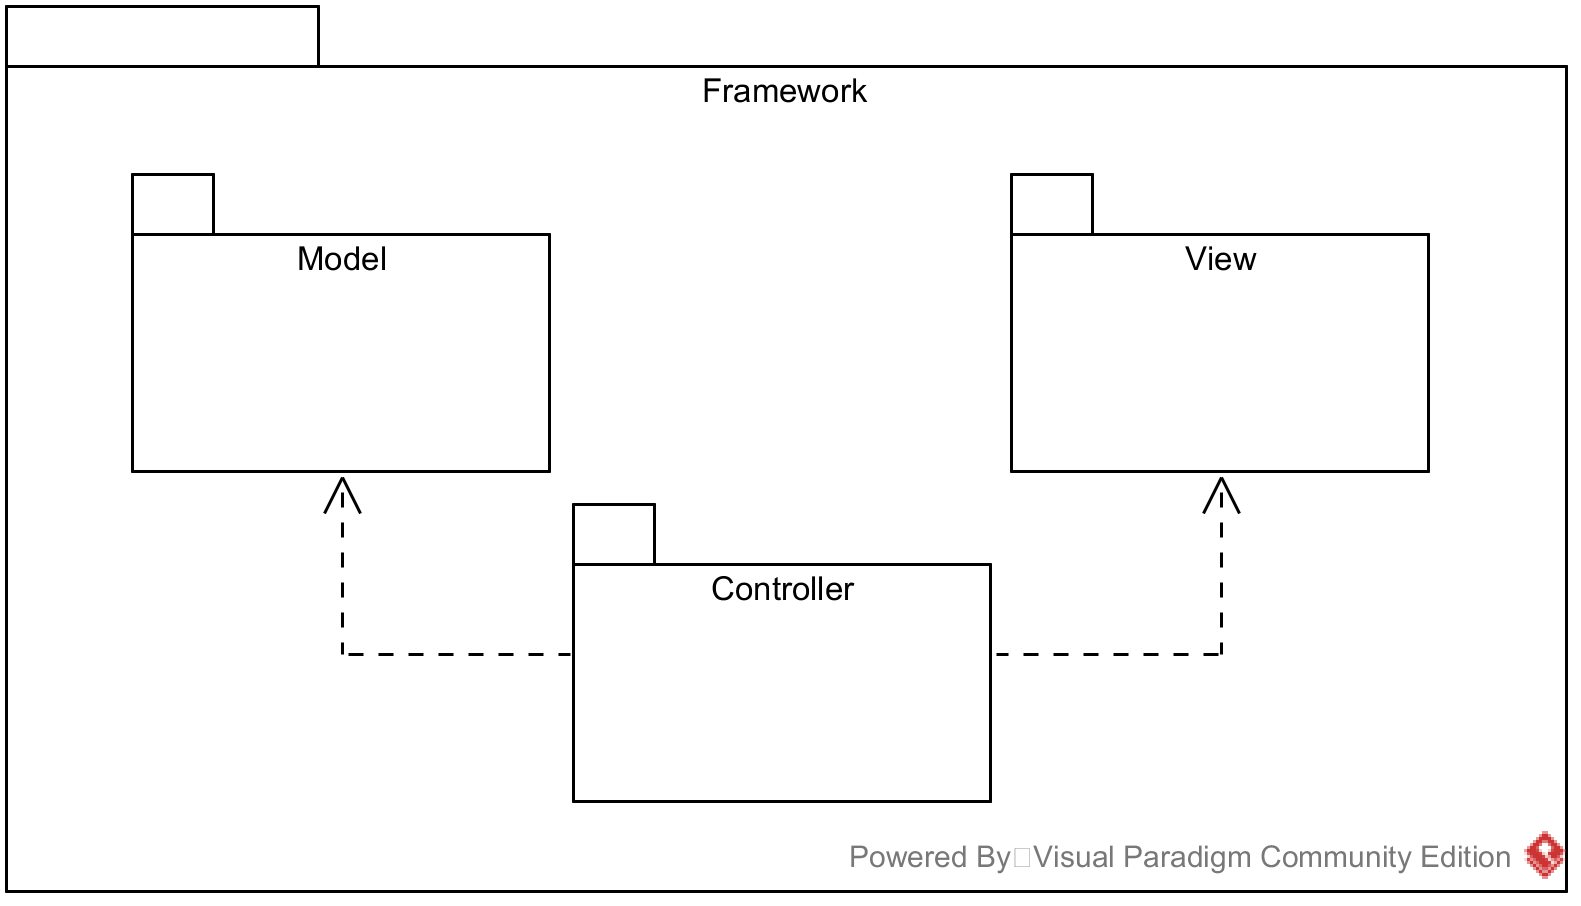
\includegraphics[width=15cm]{./diagrammi/framework.png}
%	\caption{Componente Framework}
%\end{figure}
Il package controller è composto dalla classe listItemController.


\setclass{TodoList::View::ListItems::listItemController}
\subparagraph[::listItemController]{\class}\mbox{}\\ \label{\class}
%\begin{figure}[H]
%	\centering
%	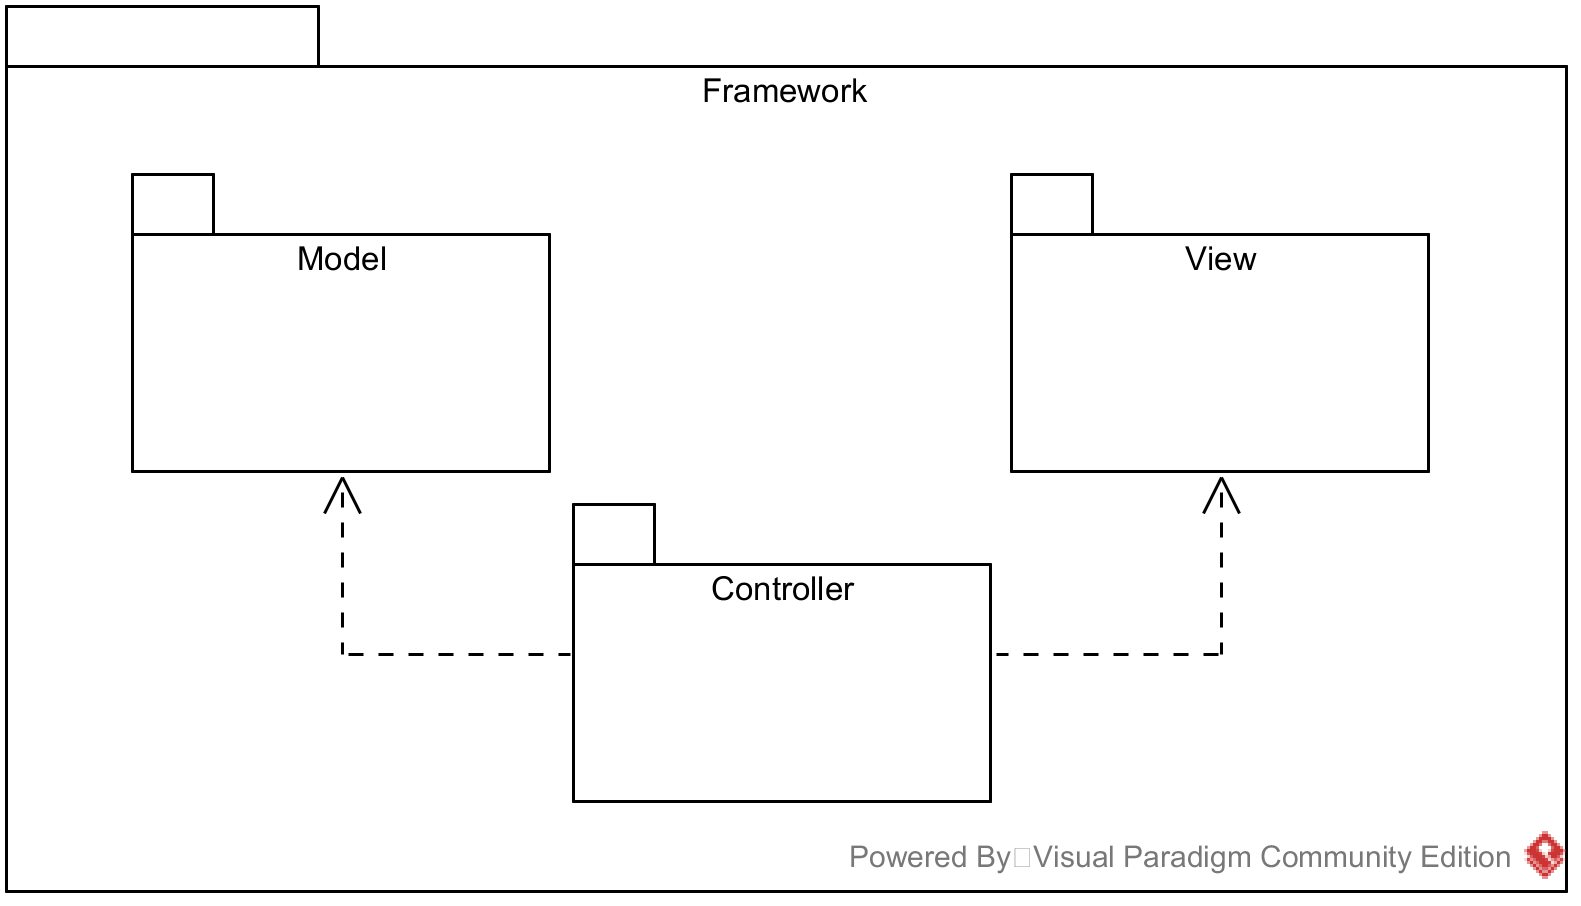
\includegraphics[width=15cm]{./diagrammi/framework.png}
%	\caption{Componente Framework}
%\end{figure}
\textbf{Descrizione:}
Questa classe rappresenta il controller della To-do list.

\textbf{Utilizzo:}
Viene utilizzata per fare da tramite tra la view e il model della To-do list.

\textbf{Classi ereditate:}
\begin{itemize}
	\item \code{React.Component};
\end{itemize}

\textbf{Attributi:}
\begin{itemize}
	\item \field{-items: listItem[]}: array contenente gli elementi della lista;
\end{itemize}

\textbf{Metodi:}
\begin{itemize}
	\item \method{+ListItemContainer()}: costruttore della classe, crea la lista recuperando i dati da TodoList::Model::ItemsStore;
	\item \method{+processInput():void}: costruisce la lista di listItem;
	\item \method{+componentWillMount()}: ricarica la lista quando viene effettuata una modifica;
	\item \method{+handleComplete():void}: comunica al model di completare un elemento della lista;
	\item \method{+handleSubmit():void}: comunica al model di aggiungere un elemento alla lista;
	\item \method{+handleRemove():void}: comunica al model di rimuovere un elemento dalla lista;
	\item \method{+render(): React.Component}: renderizza il componente.
\end{itemize}
